\section{Elektronika tlakové desky}

Tlaková plocha se díky pružné podložce a nažehlovací fólii může ve všech směrech naklánět, a díky tomu se při používání mění vzdálenost od čtyř snímacích
cívek. Tlaková plocha je primárně terčík, který slouží jako jádro cívky, která zvětšuje svou indukčnost, když se terčík přibližuje a naopak.

\begin{figure}[htbp] %todo Vodiví -> Vodivý
    \centering
    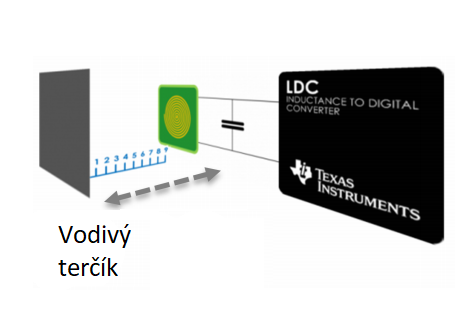
\includegraphics[width=200pt]{kapitoly/obrazky/E4/elektronika_tlakove_desky/civka_tercik_LDC.png}
    \caption{Schematické zobrazení cívky a terčíku}
    \label{fig:E4-sch_civka_tercik}
\end{figure}

Pro snímání indukčnosti používám čip \href{https://www.ti.com/lit/ds/symlink/ldc1612.pdf?ts=1612018658531&ref_url=https%253A%252F%252Fwww.google.com%252F}{LDC1614}
nebo \href{https://www.ti.com/lit/ds/symlink/ldc1312.pdf?ts=1612017390818&ref_url=https%253A%252F%252Fwww.google.com%252F}{LDC1314}, 
které se liší prakticky jen rozlišením. LDC1314 disponuje dvanáctibitovým AD převodníkem a LDC1614 dvacetiosmibitovým AD převodníkem 
a je tak schopen detekovat pohyb terčíku s rozlišením až na 10 nm.

\begin{figure}[htbp]
    \centering
    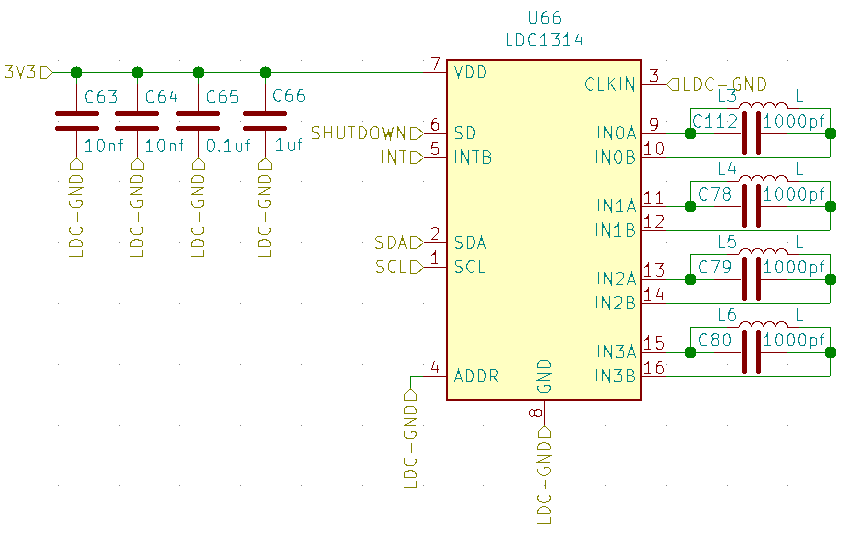
\includegraphics[width=\textwidth]{kapitoly/obrazky/E4/elektronika_tlakove_desky/moje_zapojeni.png}
    \caption{Zapojení čipu LDC1314 na desce trezoru}
    \label{fig:E4-LDC}
\end{figure}

Čip LDC komunikuje po sběrnici I2C, která umožňuje komunikaci jednoho mastera (čip, který řídí komunikaci) s až 128 slavy (čipy, které přijímají příkazy
od mastra a pouze mu odpovídají). LDC také umožňuje volbu ze dvou I2C adres, aby se daly použít dva tyto čipy na jednom I2C, nebo aby se dala změnit 
případná kolize s jiným čipem, který by měl stejnou adresu.

\newpage

Cívky použité na trezoru jsou vyrobeny jako reliéf ve vrstvě mědi přímo na DPS. Jejich vzhled jsem navrhoval v simulátoru od Texas Instruments, 
vytvořeného konkrétně pro LDC čipy, a s pomocí popisů dřívějších aplikací, které firma Texas Instruments zveřejňuje.

% obrázek ze simulátoru

Výsledná cívka je vytvořena na dvouvrstvé desce a na každé vrstvě má patnáct závitů s drahou o síle 0,152~mm se stejně velkou mezerou.

\begin{figure}[htbp]
    \centering
    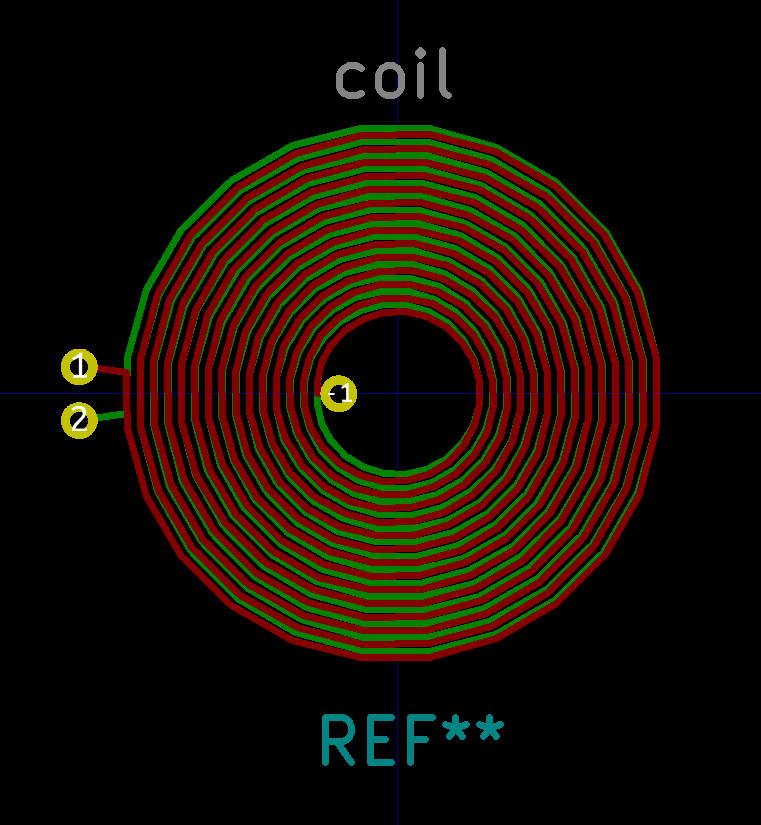
\includegraphics[width=\textwidth]{kapitoly/obrazky/E4/elektronika_tlakove_desky/civka.png}
    \caption{Vzhled reliéfu cívky}
    \label{fig:E4-relief_civka}
\end{figure}

\newpage

Celý trezor obsahuje dvě samostatné elektronické desky, přičemž na jedné je osazen jen kruh z ledek WS2812 a snímání tlakové desky, které zabírá 
většinu této desky.

\begin{figure}[htbp]
    \centering
    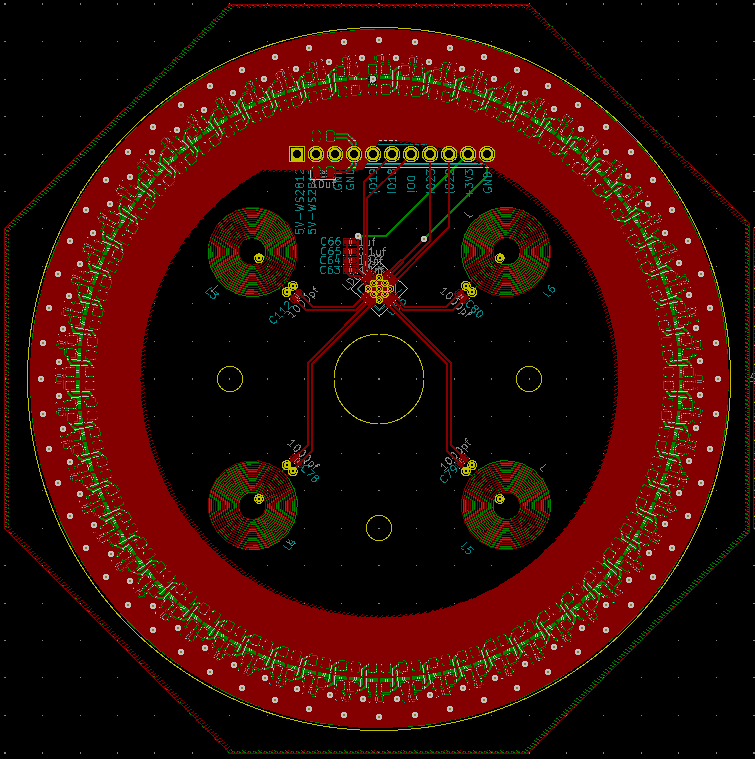
\includegraphics[width=\textwidth]{kapitoly/obrazky/E4/elektronika_tlakove_desky/leddeska-KiCad.png}
    \caption{Vzhled desky s kruhem WS2812 a snímáním tlakové desky}
    \label{fig:E4-LedDeska}
\end{figure}

\newpage